%Classe de document
\documentclass[11pt,a4paper]{scrreprt}

%%%%%%%%%%%%% Les paquetages inclus maintenant dans les style bredele: %%%%%%%%%%%%%
%Francisation
%\usepackage [latin1] {inputenc} 
%\usepackage [LGR,T1] {fontenc} % Saisie fran??ais + grec
%\usepackage [greek, frenchb] {babel}
%\usepackage[babel]{csquotes}

%R?©glages g?©n?©rauxw
%\usepackage{graphicx}
%\usepackage{textcomp} %Acc??s aux symboles Euro, etc.
%\usepackage[style=authortitle,hyperref]{biblatex}
%\usepackage{fancyhdr}
%\FrenchFootnotes
%\fancyhead[LE,RO]{\thepage}
%\fancyhead[CE]{\scshape \leftmark}

%%%%%%%%%%%%% Les paquetages divers dªsactivªs: %%%%%%%%%%%%%
%\usepackage{pxfonts}
%\usepackage{lmodern}
%\makeatletter
%\DeclareGraphicsExtensions{.pdf, .jpg, .tif, .gif}
%\AddThinSpaceBeforeFootnotes
%\fancyhead[CO]{\scshape \rightmark}
%fancyfoot[CO]{}
%\pagestyle{headings}
%\pagestyle{plain}
% En-tete
%\lhead{}        \chead{En-tte}        \rhead{}

\usepackage{tikz}
\usepackage{flupstyleutf}
\bibliography{flup}
\usepackage{harmony}
\usepackage{makeidx}
\usepackage{pdfpages}
\usepackage[colorlinks=black]{hyperref}
%\usepackage{ae}
\usepackage{musixtex}
\setlength{\parindent}{0pt} %Supprime l'indentation en début de paragraphe
\pagestyle{fancy}
\usepackage[bitstream-charter]{mathdesign}
%\usepackage{libertine}
\renewcommand*\oldstylenums[1]{{\fontfamily{fxlj}\selectfont #1}}
\usepackage{multirow}
\makeindex

\usepackage{tikz}
\usetikzlibrary{arrows}

\begin{document}
%--------------------------PAGE DE GARDE-------------------
%----------------------------------------------------------------------
\thispagestyle{empty}
\pagenumbering{roman}
\begin{center}
\begin{LARGE}
Académie de Woluwe-Saint-Pierre
\end{LARGE}
\end{center}

\begin{center}
\begin{LARGE}
\textbf{Cours de formation musicale}
\end{LARGE}
\end{center}

\begin{center}
\vspace{5cm}
\noindent\rule{\textwidth}{0.5mm}
\begin{huge}
\textbf{Aide-mémoire de théorie \\
\vspace{2 cm}
 Qualification Adultes 1 et 2}
\end{huge}
\noindent\rule{\textwidth}{0.5mm}
\end{center}

%------------------------------------INTRODUCTION--------------------
%------------------------------------------------------------------------------
%\clearpage
%\thispagestyle{empty}
%\pagenumbering{roman}
%\addcontentsline{toc}{chapter}{\numberline{}Remerciements}
%\chapter*{Remerciements}
%\begin{vcenterpage}


%\paragraph{À l'attention des parents}
%\paragraph{}
%Ce petit aide-mémoire reprend les différents notions de théorie correspondantes à chaque degré de formation musicale à l'académie. Chaque professeur expliquera ces notions à sa manière devant les élèves, mais les pages qui suivent permettent de retrouver rapidement les différents chapitres vus pendant l'année, de façon résumée mais néanmoins précise.


%\end{vcenterpage}
%--------------------------TDM ETC------------ ------------------------
%------------------------------------------------------------------------------
\newpage
\pagenumbering{roman}
\selectlanguage{french}
\lhead{Aide-mémoire de théorie}
\rhead{Qualification Adultes 1 et 2}
\fancyfoot[CO]{\thepage}%ajouter CE si a marche pas
\tableofcontents
%\sommaire
%\listoffigures
\cleardoublepage
%--------------------------CHAPITRE 1------------ ----------------
%------------------------------------------------------------------------------
%\chapter{Clés, intervalles}
\clearpage
\pagenumbering{arabic}
\lhead{Aide-mémoire de théorie}
\rhead{Qualification Adultes 1 et 2}
\fancyfoot[CO]{\thepage}%ajouter CE si ça marche pas
\chapter{Clés, intervalles}
\section{Les clés}
Il existe 3 types de clés différents\footnote{En dehors des clés de percussion et de tablatures.}:
\begin{description}
\item [clé de sol:] (2\ieme{} ligne)
\item [clés de fa:] (4\ieme{} ou 3\ieme{} ligne)
\item  [clés d'ut:] (1\iere, 2\ieme, 3\ieme{} ou 4\ieme{} ligne)
\end{description}
\begin{center}
\includegraphics{./exemples/ex_cles.pdf}
\end{center}

Chaque instrument\footnote{Chaque instrument à hauteur déterminée.} utilise une ou plusieurs clés, en fonction de son nombre de portées et de sa tessiture\index{tessiture}. Certaines clés seront donc plutôt utilisées par les instruments graves, d'autres par les instruments aigus. Ainsi le do grave en clé de sol s'écrira do aigu en clé de fa.

\centerline{\includegraphics{exemples/do_clesol_clefa.pdf}}

Actuellement on n'utilise couramment que 4 clés: clés de sol et fa, d'ut 3\ieme{} ligne (pour l'alto) et d'ut 4\ieme{} ligne (pour certaines parties de violoncelle, contrebasse, basson ou trombone). Les 3 autres sont utilisées pour la transposition (voir chapitre \ref{transpovue}) ou dans les partitions de musique ancienne.


\section{Tons et demi-tons}
Le ton est constitué de l'addition d'un demi-ton diatonique et d'un demi-ton chromatique.
\subsubsection{Le demi-ton diatonique}\index{diatonique}
Appelé également demi-ton naturel (puisque on le trouve notamment entre certaines notes naturelles, non altérées), c'est le demi-ton situé entre deux notes de noms différents. Exemples: mi -- fa ou do \fetasharp{} -- ré. Il compte 4 commas\footnote{Le comma\index{comma} est une subdivision du ton. Par convention et simplification, on considère que le ton en compte~9.}.
\subsubsection{Le demi-ton chromatique}\index{chromatique}
C'est le demi-ton situé entre 2 notes de nom identique. Il compte 5 commas. Exemple: si -- si \fetaflat


Par convention et de façon à maintenir la logique tonale, on maintient la différence écrite et logique entre ces deux demi-tons, malgré l'absence de différence sonore.
\subsubsection{Équisonance}\index{equisonance@équisonance}
L'équisonance (ou enharmonie)\index{enharmonie}: notes de même son, mais de noms différents. Exemples: si -- do \fetaflat{} ou fa \fetasharp{} -- sol~\fetaflat.

\section{Intervalles}
Un intervalle est la distance entre deux notes. Elle se calcule de plusieurs façons:
\begin{description}
\item[nom de l'intervalle:] en fonction du nombre de notes de l'intervalle (voir plus bas) 
\item[contenance:] le nombre de tons et demi-tons contenus de l'intervalle
\item[qualification:] la combinaison des 2 précédents, qui qualifie l'intervalle de majeur, mineur, juste, augmenté ou diminué
\end{description}
\subsection{Les noms d'intervalles}
\begin{description}
\item [1 note:] prime
\item [2 notes:] seconde
\item [3 notes:] tierce
\item [4 notes:] quarte
\item [5 notes:] quinte
\item [6 notes:] sixte
\item [7 notes:] septième
\item [8 notes:] octave
\end{description}

Au-delà, on parle de neuvième, dixième etc.

Remarque: on compte toujours la note de départ, celle d'arrivée et toutes celles qui sont située entre les 2.
\subsection{La contenance}\index{contenance}
Il s'agit de la quantité de tons et demi-tons contenue dans un intervalle. Attention aux additions de demi-tons!

\subsection{La qualification}
Il s'agit d'un qualificatif attribué à chaque intervalle, en fonction de son nom et de sa contenance. Il n'existe qu'un seul intervalle portant le même nom et ayant la même contenance.

Certains intervalles peuvent être \emph{majeurs} (M) ou \emph{mineurs} (m). D'autres ne peuvent l'être mais pourront être \emph{justes}. Tous les intervalles peuvent également être augmentés et diminués.

Ainsi:
\begin{enumerate}
\item quartes, quintes, octaves et primes peuvent être justes, augmentées, diminuées
\item secondes, tierces, sixtes, septièmes peuvent être majeures, mineures, augmentées, diminuées.
\end{enumerate}

De plus, la qualification d'un intervalle est inversée en cas de renversement: en renversant une sixte mineure, on obtiendra une tierce majeure, par exemple.

Voici un tableau récapitulatif des contenances et qualifications d'intervalles. Les demi-tons chromatiques sont notés \og c\fg. Sans autre précision, ils sont diatoniques.

\begin{center}
\begin{tabular}[width=15cm]{|c|c|c|c|c|c|}
\hline
Nom & diminuée & mineure & juste & majeure & augmentée\\
\hline
&&&&&\\
\multirow{2}{*} {prime} &&&\includegraphics[width= 2.35cm]{exemples/primejuste}&&\includegraphics[width= 2.35cm]{exemples/primeaug}\\
&  & &unisson &  & $\frac 1 2$ ton c\\ 
&&&&&\\ \hline
&&&&&\\
\multirow{2}{*} {seconde} &\includegraphics[width=2.35cm]{exemples/secondedim}&\includegraphics[width= 2.35cm]{exemples/secondemin}&&\includegraphics[width= 2.35cm]{exemples/secondemaj}&\includegraphics[width= 2.35cm]{exemples/secondeaug}\\
& $\frac 1 9$ ton  & $\frac 1 2$ ton d & & 1 ton & 1 ton $\frac 1 2$ c\\ 
&&&&&\\ \hline
&&&&&\\
\multirow{2}{*} {tierce} &\includegraphics[width= 2.35cm]{exemples/tiercedim}&\includegraphics[width= 2.35cm]{exemples/tiercemin}&&\includegraphics[width= 2.35cm]{exemples/tiercemaj}&\includegraphics[width= 2.35cm]{exemples/tierceaug}\\
& $\frac2 2$ d & 1 ton $\frac1 2$ d & & 2 tons & 2 tons $\frac1 2$ c\\
&&&&&\\ \hline
&&&&&\\
\multirow{2}{*} {quarte} &\includegraphics[width= 2.35cm]{exemples/quartedim}& &\includegraphics[width= 2.35cm]{exemples/quartejuste}&&\includegraphics[width= 2.35cm]{exemples/quarteaug}\\
& 1 ton $\frac2 2$ d & & 2 tons $\frac1 2$ d & & 3 tons\\
&&&&&\\ \hline
&&&&&\\
\multirow{2}{*} {quinte} &\includegraphics[width= 2.35cm]{exemples/quintedim}& &\includegraphics[width= 2.35cm]{exemples/quintejuste}&&\includegraphics[width= 2.35cm]{exemples/quinteaug}\\
& 2 tons $\frac2 2$ d & & 3 tons $\frac1 2$ d & & 4 tons\\
&&&&&\\ \hline
&&&&&\\
\multirow{2}{*} {sixte} &\includegraphics[width= 2.35cm]{exemples/sixtedim}&\includegraphics[width= 2.35cm]{exemples/sixtemin}&&\includegraphics[width= 2.35cm]{exemples/sixtemaj}&\includegraphics[width= 2.35cm]{exemples/sixteaug}\\
& 2 tons $\frac3 2$ d & 3 tons $\frac2 2$ d & & 4 tons $\frac1 2$ d & 5 tons\\
&&&&&\\ \hline
&&&&&\\
\multirow{2}{*} {septième} &\includegraphics[width= 2.35cm]{exemples/septdim}&\includegraphics[width= 2.35cm]{exemples/septmin}&&\includegraphics[width= 2.35cm]{exemples/septmaj}&\includegraphics[width= 2.35cm]{exemples/septaug}\\
& 3 tons $\frac3 2$ d & 4 tons $\frac2 2$ d& & 5 tons $\frac12$ d & 6 tons\\
&&&&&\\ \hline
&&&&&\\
\multirow{2}{*} {octave} &\includegraphics[width= 2.35cm]{exemples/octavedim}& &\includegraphics[width= 2.35cm]{exemples/octavejuste}&&\includegraphics[width= 2.35cm]{exemples/octaveaug}\\
& 4 tons $\frac3 2$ d & & 5 tons $\frac2 2$ d & & 6 tons $\frac12$ d\\
&&&&&\\
\hline
\end{tabular}
\end{center}


\subsection{Le renversement}\index{renversement}
Un intervalle peut-être renversé: on fait passer une des 2 notes par-dessus ou par-dessous l'autre, sans changer le nom des notes. La qualification d'un intervalle est inversée en cas de renversement. Exemple: en renversant une sixte mineure, on obtiendra une tierce majeure.

\centerline{\includegraphics[width=5cm]{exemples/renversement}}

On rencontrera les reversements suivants :
%\begin{itemize}
%\item seconde $\longleftrightarrow$ septième
%\item tierce $\longleftrightarrow$ sixte
%\item quarte $\longleftrightarrow$ quinte
%\item octave $\longleftrightarrow$ quinte
%\end{itemize}

\vspace{0.5cm}
\begin{center}
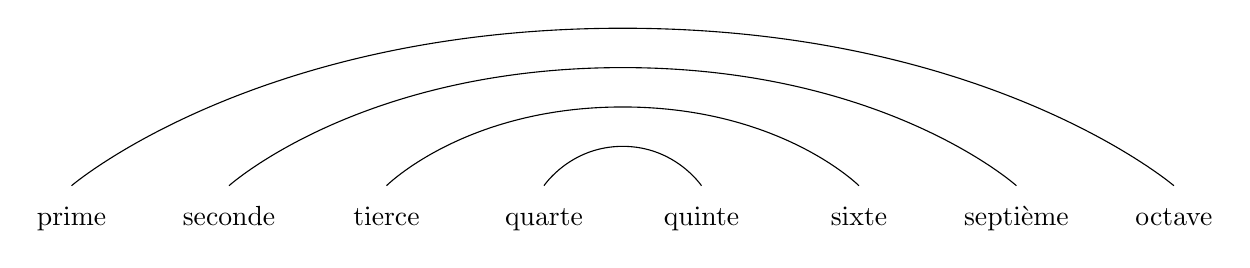
\begin{tikzpicture}{anchor=base}
	\tikzstyle{lettre}=[anchor=base]
	\node[lettre] (A) at (0,0){prime};
	\node[lettre] (B) at (2,0){seconde};
	\node[lettre] (C) at (4,0){tierce};
	\node[lettre] (D) at (6,0){quarte};
	\node[lettre] (E) at (8,0){quinte};
	\node[lettre] (F) at (10,0){sixte};
	\node[lettre] (G) at (12,0){septième};
	\node[lettre] (H) at (14,0){octave};
%	\draw[fleche] (A) -- (H);
%	\path (A) edge node [above] (B);
%	\draw (A) -- (H) arc (2:170:7 and 4);
%	\draw (B) -- (G) arc (2:170:5 and 3);
%	\draw (C) -- (F) arc (2:170:3 and 2);
\draw[black] plot [smooth, tension=1.2]  coordinates {(0,0.5)  (7,2.5) (14,0.5)};
\draw[black] plot [smooth, tension=1.2]  coordinates {(2,0.5)  (7,2) (12,0.5)};
\draw[black] plot [smooth, tension=1.2]  coordinates {(4,0.5)  (7,1.5) (10,0.5)};
\draw[black] plot [smooth, tension=1.2]  coordinates {(6,0.5)  (7,1) (8,0.5)};


%	\node (A) at (0,0){prime};
%	\node (B) at (2,0){seconde};
%	\node (C) at (4,0){tierce};
%	\node (D) at (6,0){quarte};
%	\node (E) at (8,0){quinte};
%	\node (F) at (10,0){sixte};
%	\node (G) at (12,0){septième};
%	\node (H) at (14,0){octave};
%	\path (A) edge (B);
	%\draw (A) -- (H) arc (-10:180:7 and 2);


\end{tikzpicture}
\end{center}




\subsection{Le redoublement}\index{redoublement}
Un intervalle redoublé est un intervalle plus grand qu'une octave. Sa qualification se calcule en ne tenant compte que de l'intervalle dépassant l'octave juste. Exemple: une neuvième de 6 tons et $\frac2 2$ aura la même qualification qu'une seconde de 1 ton.\\

\chapter{Gammes, tonalités}
\section{Degrés}\index{degré}
Chaque note dans la gamme porte un nom, en fonction de sa place. 
\begin{itemize}
\item I: tonique
\item II: sus-tonique
\item III: médiante
\item IV: sous-dominante
\item V: dominante
\item VI: sus-dominante
\item VII: sensible
\end{itemize}
En mineur antique (voir \ref{min_ant}), la septième note de la gamme porte le nom de sous-tonique, étant donné qu'il y a un ton et non $\frac1 2$ entre cette dernière et la tonique. Les degrés de la gamme se notent de chiffres romains.
\section{Armures}\index{armure}
Les altérations présentes à l'armure se présentent toujours dans un ordre précis\footnote{Dans les limites du système tonal (majeur~--~mineur). Certains compositeurs sortent de ce système et utilisent donc d'autres ordres.}.
\subsubsection{Ordre des dièses}
FA DO SOL RÉ LA MI SI
\subsubsection{Ordre des bémols}
SI MI LA RÉ SOL DO FA
\\
\\
Cette armure permet de déterminer la tonalité majeure ou mineure présente dans une partition. À chaque armure correspondent 2 tonalités: une majeure, l'autre mineure. Par facilité, on calcule d'abord la possibilité majeure, avant de calculer la relative mineure.

\subsubsection{Tonalités en dièse}
Le dernier dièse présent à l'armure correspond à la sensible de la tonalité majeure. Il suffit juste de monter d'$\frac1 2$ ton diatonique à partir de cette note (qui est toujours un \fetasharp{}) pour obtenir le nom de la tonalité majeure)
\subsubsection{Tonalités en bémols}
La tonique correspond à l'avant-dernier \fetaflat. Exception: Fa Majeur, dont l'armure est si \fetaflat{} (puisqu'il n'y a pas dans ce cas d'avant-dernier \fetaflat).
\section{Gammes}
Une gamme est une suite d'intervalle. Elle peut être transposée à partir de n'importe quelle note, pour peu que les intervalles soient respectés dans leur contenance et leur ordre d'origine. Il existe de nombreuses gammes et le nombre de notes qu'elles contiennent est assez varié.
\section{Tonalité et modes}
Les deux modes les plus connus sont les modes majeur  et mineur. Ils ont acquis une importance telle qu'on en est arrivé à considérer tout autre gamme comme étant une variante du majeur ou du mineur.
\subsection{La gamme majeure}\index{gamme!majeure}
\begin{center}
  \includegraphics{exemples/gamme_maj.pdf}
\end{center}
Elle est construite sur le schéma suivant: 
\begin{center}
\fbox{1t - 1t - $\frac1 2$t - 1t - 1t - 1t - $\frac1 2$t}
\end{center}


\subsection{La gamme mineure}
La gamme mineure possède plusieurs formes couramment utilisées. Toutes sont malgré tout basées sur la gamme mineure "antique", qui est la seule à correspondre à son armure.

\subsubsection{Gamme mineure antique\label{min_ant}}\index{gamme!mineure antique}
\begin{center}
   \includegraphics{exemples/gamme_min_ant.pdf}
\end{center}

Elle est construite sur le schéma suivant: 
\begin{center}
\fbox{1t - $\frac1 2$t - 1t - 1t - $\frac1 2$t - 1t - 1t}
\end{center}
Le 7\ieme{} degré est ici appelé "sous-tonique" et non "sensible", vu qu'il y a 1 ton entre cette note et la tonique.

\subsubsection{Gamme mineure harmonique}\index{gamme!mineure harmonique}
\begin{center}
   \includegraphics{exemples/gamme_min_har.pdf}
\end{center}

Pour pallier l'absence de sensible, cette gamme présente un 7\ieme{} degré haussé, devenant ainsi une sensible. Par contre, l'intervalle VI - VII d'1 ton $\frac1 2$ (seconde augmenté) rend cette gamme peu chantante. Son nom "harmonique" indique d'ailleurs qu'elle est utilisée pour constituer l'harmonie et les accords d'une musique.

Elle est construite sur le schéma suivant: 
\begin{center}
\fbox{1t - $\frac1 2$t - 1t - 1t - $\frac1 2$t - 1t $\frac1 2$ - $\frac1 2$t}
\end{center}

\subsubsection{Gamme mineure mélodique}\index{gamme!mineure mélodique}
Tout en conservant la sensible introduite dans la gamme mineure harmonique, elle rétablit l'intervalle VI - VII d'1 ton, rendant la gamme beaucoup plus adaptée à l'écriture mélodique. Cette gamme, contrairement aux autres, possède une forme descendante différente de la forme ascendante, et qui est similaire à la gamme antique.

Elle est construite sur le schéma suivant: 
\begin{center}
\fbox{1t - $\frac1 2$t - 1t - 1t - 1t - 1t  - $\frac1 2$t}
\end{center}
\begin{center}
   \includegraphics{exemples/gamme_min_mel.pdf}
\end{center}

%\begin{center}
%\includegraphics{exemples/horloge}
%\includegraphics{exemples/horlogemin}
%\end{center}
%%%%%%%%%%CYCLE DES QUINTES%%%%%%%%%%%
\begin{center}
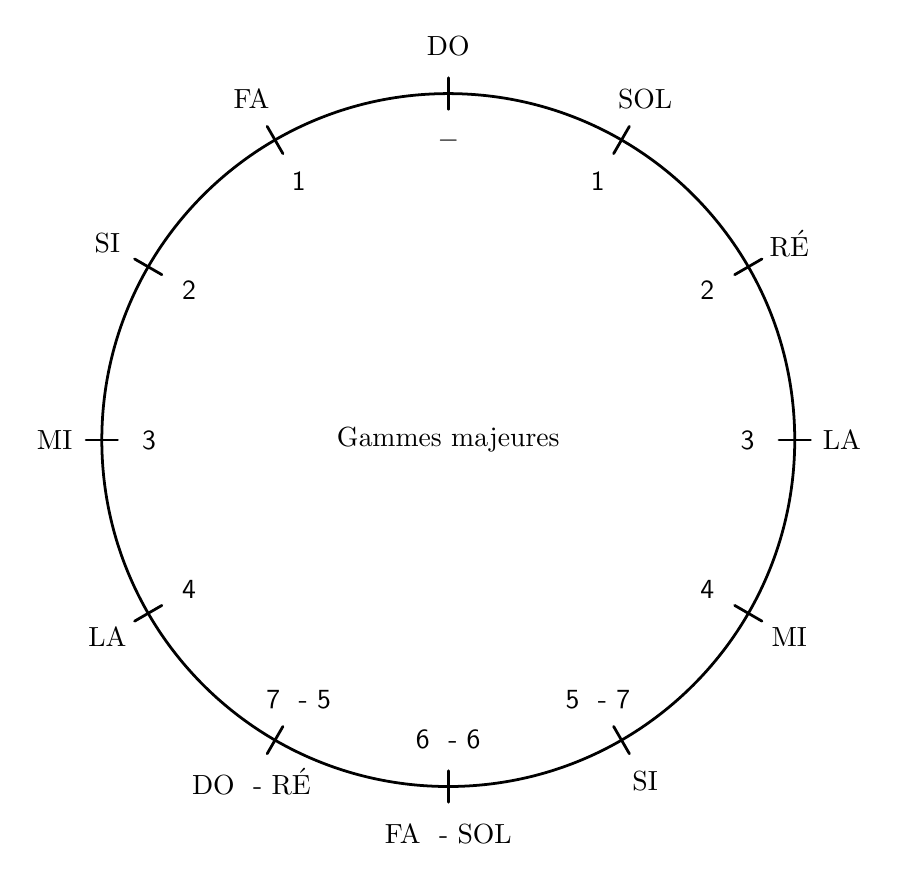
\begin{tikzpicture} [line cap=round,line width=1pt] 
\draw (0,0) circle (4.4cm);

\foreach \angle / \label in 
{0/{LA}, 30/{RÉ}, 60/{SOL}, 90/{DO}, 120/{FA}, 150/{SI \fetaflat}, 180/{MI \fetaflat},
210/{LA \fetaflat}, 240/{DO \fetasharp{} - RÉ \fetaflat}, 270/{FA \fetasharp{} - SOL \fetaflat}, 300/{SI}, 330/{MI}}
{
\draw[line width=1pt] (\angle:4.2cm) -- (\angle:4.6cm); 
\draw (\angle:5.0cm) node{\label};
}
\foreach \angle / \label in 
{0/{3 \fetasharp}, 30/{2 \fetasharp}, 60/{1 \fetasharp}, 90/{$-$}, 120/{1 \fetaflat}, 150/{2 \fetaflat}, 180/{3 \fetaflat},
210/{4 \fetaflat}, 240/{7 \fetasharp{} - 5 \fetaflat}, 270/{6 \fetasharp{} - 6 \fetaflat}, 300/{5 \fetasharp{} - 7 \fetaflat}, 330/{4 \fetasharp}}
{
\draw (\angle:3.8cm) node{\textsf{\label}};
}
\node (0,0){Gammes majeures};
\end{tikzpicture}
\end{center}

\begin{center}
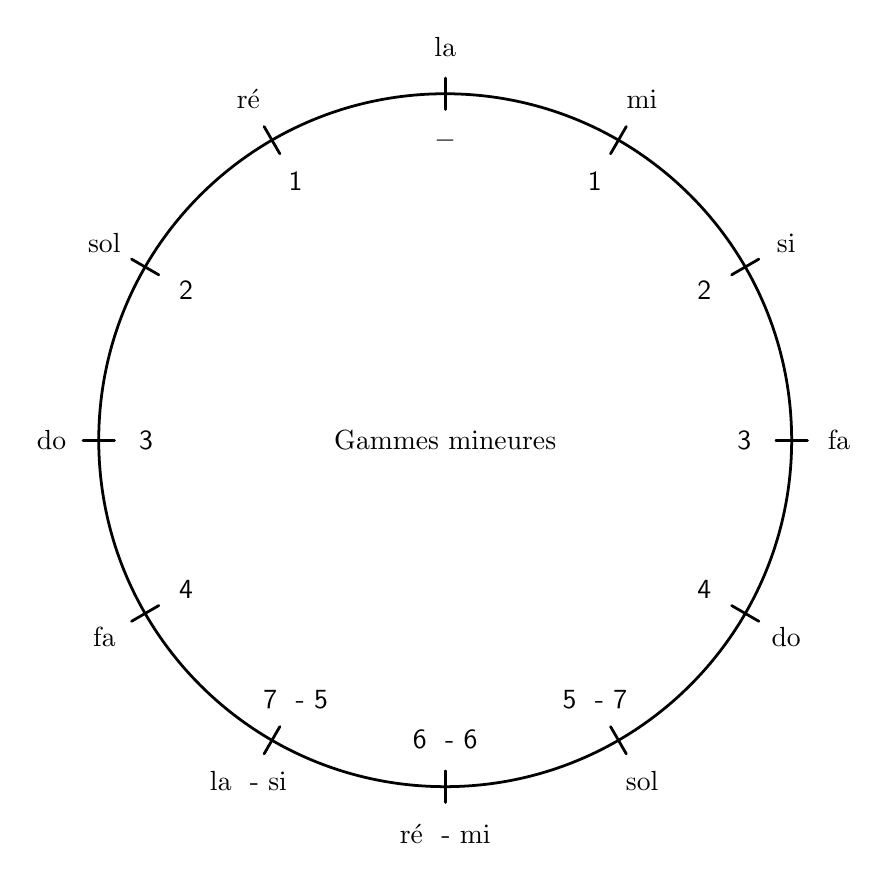
\begin{tikzpicture} [line cap=round,line width=1pt] 
\draw (0,0) circle (4.4cm);

\foreach \angle / \label in 
{0/{fa \fetasharp}, 30/{si}, 60/{mi}, 90/{la}, 120/{ré}, 150/{sol}, 180/{do},
210/{fa}, 240/{la \fetasharp{} - si \fetaflat}, 270/{ré \fetasharp{} - mi \fetaflat}, 300/{sol \fetasharp}, 330/{do \fetasharp}}
{
\draw[line width=1pt] (\angle:4.2cm) -- (\angle:4.6cm); 
\draw (\angle:5.0cm) node{\label};
}
\foreach \angle / \label in 
{0/{3 \fetasharp}, 30/{2 \fetasharp}, 60/{1 \fetasharp}, 90/{$-$}, 120/{1 \fetaflat}, 150/{2 \fetaflat}, 180/{3 \fetaflat},
210/{4 \fetaflat}, 240/{7 \fetasharp{} - 5 \fetaflat}, 270/{6 \fetasharp{} - 6 \fetaflat}, 300/{5 \fetasharp{} - 7 \fetaflat}, 330/{4 \fetasharp}}
{
\draw (\angle:3.8cm) node{\textsf{\label}};
}
\node (0,0){Gammes mineures};
\end{tikzpicture}
\end{center}

D'autres gammes \index{gamme!(autres)}sont souvent associées aux gammes mineures (gamme mixte, gamme bohémienne, gamme  orientale) mais il est plus logique de les considérer comme des modes à part entière\footnote{L'aberration consistant à considérer la gamme mixte comme gamme mineure -- alors que son accord parfait est majeur -- est un exemple parmi d'autres.}.\\

Les autres modes ont malgré tout gardé une certaine importance, variable selon les époques et les lieux (musique populaire, jazz, musiques du monde etc.).

À titre d'exemple, on pourrait citer :
\begin{itemize}
\item les différentes gammes issues des modes d'église (dorien, phrygien, etc. Voir plus bas)
\item la gamme par tons
\item la gamme pentatonique
\end{itemize}

\subsection{Les modes dit \og d'église \fg}\index{modes}
Les modes d'église sont des modes issus de la musique du moyen âge et dont la terminologie est d'inspiration grecque. Pour retrouver leurs intervalles, il suffit de partir des touches blanches d'un piano (do - ré - mi - fa - sol - la - si). En fonction de la note de départ, on obtiendra un de ces modes:

\begin{enumerate}
\item do: ionien (correspond au mode majeur)
\item ré: dorien
\item mi: phrygien
\item fa: lydien
\item sol: mixolydien
\item la: éolien (correspond au mode mineur antique)
\item si: locrien
\end{enumerate}


On parlera également de \og mode de ré\fg pour le dorien, etc.


\chapter{Accords}
Un accord est une superposition d'intervalles. Le nombre d'intervalles et leur nature déterminera la couleur de l'accord. On analyse un accord en l'observant de bas en haut.

Chaque accord se présente sous la forme d'un état fondamental, mais l'ordre des notes peut être modifié; on parle alors de reversement. C'est la note la plus grave qui déterminera s'il s'agit de l'état fondamental ou d'un renversement.
\section{Accords de 3 sons}
\subsection{Accords parfaits}\index{accord!parfait}
Les accords parfaits majeur et mineur sont constitués d'une tierce M et d'une tierce m.
\begin{center}
   \includegraphics{exemples/accpft.pdf}
\end{center}


\subsubsection{Accord parfait majeur}\label{pftmaj}
La tierce inférieure est majeure, l'autre mineure.

\subsubsection{Accord parfait mineur}
La tierce inférieure est mineure, l'autre majeure.

\subsection{Accord de quinte diminuée}\index{accord!de quinte diminuée}
Cet accord est composé de 2 tierces mineures, formant au total une quinte diminuée (2 tons et $\frac2 2$)
\begin{center}
   \includegraphics{exemples/acc3sons.pdf}
\end{center}
\subsection{Accord de quinte augmentée}\index{accord!de quinte augmentée}
Il est constitué de 2 tierces majeures, formant au total une quinte augmentée (4 tons). Cet accord se rencontre en mineur. La note située à distance de quinte de la fondamentale constitue la sensible; on peut donc en déduire la tonique\footnote{Le signe + devant la quinte n'indique pas nécessairement un intervalle augmenté, mais bien la sensible.}.
\section{Accords de 4 sons}
\subsection{Accord de septième de dominante}\index{accord!de septième de dominante}
Cet accord, présent tant en majeur qu'en mineur (sauf mineur antique), se forme sur la dominante d'une tonalité. On peut donc en déduire la tonique. Il est composé d'un accord parfait majeur (voir \ref{pftmaj}) et d'une tierce mineure.
\begin{center}
   \includegraphics{exemples/acc4sons.pdf}
\end{center}
\subsection{Accord de septième diminuée}\index{accord!de septième de diminuée}
Il se construit sur la sensible d'une tonalité mineure et est constitué de 3 tierces mineures. Si on ajoute une 4e tierce mineure à cet accord, on obtient une enharmonie\index{enharmonie} de la fondamentale. Il est ainsi possible d'écrire un accord de 7\ieme{} diminuée par enharmonie; on obtient ainsi des accords appartenant à des tonalités différentes malgré un résultat sonore identique.
\section{Analyse harmonique}
La fonction harmonique d'un accord tient à sa composition, et non à la position (renversée ou non) dans laquelle on le rencontre; il y aura donc toujours lieu de le replacer à l'état fondamental de façon à l'analyser, et donc à déterminer avec certitude sa fonction dans la structure harmonique. À l'état fondamental, c'est la note la plus basse qui servira de base au calcul.
\subsection{Arpèges}\index{arpège}
Un arpège consiste en un accord dont les notes ne sont pas jouées simultanément, mais successivement. Il s'analyse malgré tout comme un accord. Les instruments harmoniques\footnote{Les instruments qui sont capables de jouer plusieurs notes simultanément.} ne sont donc pas les seuls à jouer des accords.

%--------------------------CADENCES ET MODULATIONS---------------------
%------------------------------------------------------------------------------
\chapter{Cadences et modulations}
\section{Cadences}\index{cadence}
Une cadence est un enchaînement d'accords. La succession des fonctions harmoniques représentées par les accords produira un effet différent; ces enchaînements différents auront donc des usages différents\footnote{Tous les exemples qui suivent sont en Do Majeur.}. Ainsi, on compare très souvent les cadences à la ponctuation d'un texte (point final, point-virgule, etc.)
\subsection{Cadence parfaite}
La cadence parfaite est constituée d'une dominante suivie d'une tonique, les 2 étant à l'état fondamental. C'est la cadence conclusive et affirmative par excellence.
\begin{center}
  \includegraphics{exemples/cadence_pft.pdf}
\end{center}
\subsection{Cadence imparfaite}
Elle reprend les mêmes fonctions que la cadence parfaite, mais un des deux accords (au moins) se présentera sous forme d'un reversement. Elle est moins affirmative de la tonalité.
\begin{center}
   \includegraphics{exemples/cadence_impft.pdf}
\end{center}
\subsection{Cadence plagale}
Elle est composée d'une sous-dominante et d'une tonique. L'absence de sensible induit une absence de tension, ainsi qu'un caractère modale.
\begin{center}
   \includegraphics{exemples/cadence_plag.pdf}
\end{center}
\subsection{Demi-cadence}
Elle est composée d'une tonique suivie d'une dominante; c'est donc le contraire des cadences parfaite et imparfaite. Elle s'utilise souvent lors d'un repos sur la dominante.
\begin{center}
   \includegraphics{exemples/cadence_demi.pdf}
\end{center}
\subsection{Cadence rompue}
Elle est composée d'une dominante suivie de n'importe quelle autre fonction à l'exception de la tonique; elle crée un effet de surprise, généré par l'attente d'une tonique qui ne vient finalement pas.
\begin{center}
   \includegraphics{exemples/cadence_romp.pdf}
\end{center}

Note: on parle parfois de cadence évitée. Certains théoriciens considèrent la cadence rompue (V $\to$ VI) comme un cas particulier de la cadence évitée (V $\to$ \emph{autre chose que I} ).
\section{Modulation}\index{modulation}
La modulation correspond au changement de tonalité; elle peut être passagère ou durable, préparée ou brutale. Les modulations les plus simples se font par tonalités voisines, le nombre de notes communes entre ces tonalités étant important.
\subsection{Tons voisins}\index{tons voisins}
Les tons voisins sont les tonalités ou gammes qui ont un grand nombre de notes en commun, et donc des armures très proches. Les tonalités voisines sont distantes d'une quinte juste; il est donc possible, par simple calcul, de déterminer les tonalités dont les armures sont proches. À partir de là, on peut faire de même avec les relatifs mineurs, puisque chaque armure est partagée par une tonalité majeure et une tonalité mineure, séparées par une tierce mineure. Dans la tableau suivant, les $\to$ indiquent des quinte justes montantes, les~$\leftarrow$ des quintes justes descendantes, les $\downarrow$ des tierces mineures descendantes et les parenthèses indiquent la sensible des tons mineurs.

\begin{center}
\begin{tabular}{ccccc}
Fa Majeur & $\leftarrow$ & Do Majeur & $\to$ & Sol Majeur \\
&&&&\\
1 \fetaflat & & \fetanatural & & 1 \fetasharp\\
&&&&\\
$\downarrow$ & & $\downarrow$ & & $\downarrow$ \\
&&&&\\
ré mineur & $\leftarrow$ & la mineur & $\to$ & mi mineur\\
&&&&\\
(do \fetasharp) &$\leftarrow$ & (sol \fetasharp) &$\to$ & (ré \fetasharp)\\
&&&&\\
&&&&\\
&&Ton direct: Do mineur&&\\
\label{tonsvoisins}
\end{tabular}
\end{center}


\subsubsection{Ton direct}
Le ton direct n'est pas à proprement parler un ton proche du point de vue de l'armure, mais il partage la même tonique avec le ton de départ. À ce titre, son utilisation est très courante\footnote{Exemple: l'Introduction d'\emph{Also sprach Zarathustra} de Richard Strauss, entendue au début du film \emph{2001, A space Odyssey} de Stanley Kubrik}. Rappelons d'ailleurs qu'il n'y a qu'une note de différence entre une gamme mineure mélodique et son ton direct majeur.

%--------------------------TRANSPOSITION------------ ------------------------
%------------------------------------------------------------------------------
\chapter{Transposition\index{transposition}}
\section{Transposition écrite\index{transposition!écrite}}
Il s'agit simplement de transcrire une partition en appliquant à chaque note le même intervalle. L'intervalle entre les notes de la partition sera ainsi respecté \footnote{On pourrait comparer cela à un translation de vecteur $\vec v$ où $v$ correspond à l'intervalle de transposition.}.
\section{Transposition à vue}\label{transpovue}\index{transposition!à vue}
La transposition à vue permet d'exécuter une partition en la transposant séance tenante, sans retranscription écrite préalable. Elle fait appel à de nombreuses notions théoriques (tonalités, armures, intervalles, etc.). La marche à suivre -- à adapter en fonction des données présentes -- est grosso modo la suivante:
\begin{enumerate}
\item déterminer, si nécessaire, les tonalités jouées et entendues
\item déterminer la tonalité dans laquelle il faudra transposer, ainsi que son armure
\item déterminer la clé à utiliser pour réaliser cette transposition
\item déterminer quelles seront les mutations d'altérations accidentelles
\end{enumerate}
\subsection{Tonalité jouée ou entendue}
En fonction de l'énoncé du problème, nous connaissons la tonalité entendue (celle de l'oeuvre, qui est également celle des instruments en ut) ou la tonalité écrite (si on part de la partition d'un instrument transpositeur). Dans ce dernier cas, il faut d'abord calculer la tonalité entendue, en appliquant à la tonalité écrite l'intervalle de transposition propre à l'instrument écrit.

\subsection{Tonalité de transposition}
En fonction de la tonalité entendue, il faut calculer la tonalité utilisée par l'instrument qui doit transposer. S'il s'agit d'un instrument en ut, cette tonalité sera la tonalité entendue. Dans le cas d'un instrument transpositeur, il faudra calculer la tonalité qu'il devra jouer pour faire entendre la tonalité entendue.

\subsection{Clé de transposition}
La recherche de la nouvelle clé de fait entre la tonalité écrite de départ et la nouvelle tonalité. Cette dernière devra cependant être écrite avec une note repère à même hauteur que l'autre, puisque le changement de clé fera en sorte que les notes sonnent de façon différente sans devoir être ré-écrites.

\subsection{Mutations d'altérations}\index{mutations d'altérations}
Suite à la transposition, certaines altérations accidentelles seront modifiées.
\subsubsection{Nombre d'altérations concernées}
Pour obtenir le nombre d'altérations mutantes, on compare les 2 armures (l'armure écrite et l'armure transposée); il y a deux possibilités:
\begin{itemize}
\item les altérations des 2 armures sont de même type (\fetaflat{} dans les 2 cas par exemple): on les soustrait
\item les altérations des 2 armures sont de types différents (\fetaflat{} pour l'une, \fetasharp{} pour l'autre): on les additionne.
\end{itemize}
\subsubsection{Sens de la mutation}
On regarde ensuite les positions comparées des 2 tonalités dans le cycle des quintes. Si, pour passer de l'une à l'autre, on va: 
\begin{description}
\item [vers les dièses:] les mutations se feront vers le haut
\item [vers les bémols:] les mutations se feront vers le bas.
\end{description}
\subsubsection{Notes mutées}
Les notes subissant les mutations seront modifiées d'$\frac12$ ton chromatique. Si elles sont modifiées vers le haut, on prendra les notes concernées dans l'ordre des dièses. Si elles descendent, dans l'ordre des bémols.

%--------------------------RYTHMES------------------------------------
%------------------------------------------------------------------------------
\chapter{Rythmes et métrique}
\section{Chiffres indicateurs de mesure}
Les chiffres indiquant la mesure sont constitués de 2 nombres:
\begin{itemize}
\item le nombre supérieur indique le nombre de pulsation de la mesure
\item le nombre inférieur la valeur rythmique correspondant à cette pulsation.
\end{itemize}

Pour savoir à quelle valeur de note correspond le deuxième nombre, on divise une ronde:
\begin{itemize}
\item 1 = une ronde
\item 2 = une blanche (la moitié d'une ronde)
\item 4 = une noire (le quart d'une ronde)
\item 8 = une croche (le huitième d'une ronde)
\end{itemize}
Une mesure \metric{2}{4} indiquera donc 2 temps par mesure, chaque temps valant une noire. Une mesure \metric{2}{2} indiquera aussi 2 temps par mesure, mais chaque temps vaudra alors une blanche.

\section{Mesures binaires, ternaires et asymétriques}
\subsection{Mesures binaires}
Les mesures binaires sont les mesures dont les temps sont divisibles par 2: \metric{2}{4}, \metric{3}{4}, \metric{4}{4}, etc. On les appelle aussi \emph{mesures simples}.

\subsection{Mesures ternaires}
Les mesures ternaires sont les mesures dont les temps sont divisibles par 3: \metric{6}{8}, \metric{9}{8}, \metric{12}{8}, etc. Même si \metric{6}{8} indique une mesure de 6 croches, il ne s'agit généralement pas d'une mesure à 6 temps (sauf en tempo lent), mais d'une mesure à 2 temps, chaque temps valant 3 croches. On les appelle aussi \emph{mesures composées}

\subsection{Mesure asymétriques}
Les mesure asymétriques sont les mesures dont les temps n'ont pas tous la même durée. En mesure \metric{7}{8} par exemple, il n'est pas possible de grouper les croches de façon égale sur chaque temps; certains seront donc plus longs que d'autres. La façon dont seront groupées les croches indiquera la valeur des différents temps. Certains compositeurs le précisent, en utilisant une notation de ce genre: \metric{3+2+2}{8}.

\section{Groupes irréguliers}
Ils consistent à placer rythmiquement un groupe de notes qui ne correspond pas à une division normale de la pulsation. Le triolet est l'exemple le plus connu: 3 notes sur le temps de 2 notes \emph{normales}.
Il n'existe en français aucun terme à la fois concis et précis pour désigner ces groupements rythmiques; certains logiciels informatiques utilisent le terme \emph{n}-olet (avec \emph{n} égal à n'importe quel nombre entier). En anglais, on parle de \emph{tuplet}.

Pour éviter la confusion en fonction des équivalences possibles, les compositeurs utilisent de plus en plus souvent une notation indiquant l'équivalence complète: \emph{3 : 2} au lieu de \emph{3}.

\section{Rythmes particuliers}
\subsection{Syncope}\index{syncope}
Un syncope est formée, dans son sens le plus général, par une note placée sur un temps faible (ou la partie faible d'un temps) et qui se prolonge sur le temps suivant. 
\subsection{Contretemps}\index{contretemps}
Comme le syncope, le contretemps commence sur un temps faible ou la partie faible d'un temps, mais ne se prolonge pas.
\subsection{Hémiole}\index{hemiole@hémiole}
L'hémiole consiste à donner l'impression, dans une mesure à trois temps ou une structure ternaire, qu'on a affaire à 3 mesures de 2 temps, plutôt qu'à 2 mesures de 3 temps. Ce procédé, très courant dans la musique baroque (ou dans les mouvements de valse), donne une impression d'accélération.

\section{Silence multi-mesures}
Certains instruments doivent parfois arrêter de jouer pendant plusieurs mesures. Pour faciliter le comptage, on rassemble ces mesures en une seule en indiquant le nombre de mesures à compter.

\section{La barre de reprise}
Pour indiquer qu'il faut répéter une ou plusieurs mesures, on utilise parfois des barres de reprises. Toutes les mesures comprise entre 2 barres de reprises (ou entre le début et une barre de reprise) doivent être rejouées. Cela permet de ne pas devoir ré-écrire un passage complet et d'économiser de la place.

\includegraphics{exemples/reprise}


%--------------------------TERMES ITALIENS----------------------------------
%------------------------------------------------------------------------------
\chapter{Termes italiens, signes divers}
\section{Indications de mouvement}
Du plus lent au plus rapide:


\begin{description}
\item Lento: lent
\item Adagio: à l'aise
\item Andante: allant
\item Moderato: modéré
\item Allegretto: joyeux, rapide (mais moins qu'\emph{allegro})
\item Allegro: joyeux, rapide
\item Vivace: vif
\item Presto: très rapide
\end{description}

\section{Indications de nuances}
\begin{description}
\item \fetap : doux, doucement (piano)
\item \fetamp : modérément doux (mezzo piano)
\item \fetamf : modérément fort (mezzo forte)
\item \fetaf : fort (forte)
\item \fetasfz : sforzando (en renforçant une note)
\item Crescendo\index{crescendo} (<): en augmentant l'intensité du son
\item Decrescendo\index{decrescendo} (>): en diminuant l'intensité du son
\end{description}

\section{Symboles et signes divers}
\begin{description}
\item \fetasegno : il faut reprendre à l'endroit où ce signe a déjà été vu
\item \fetacoda : indique une \emph{coda}, un passage de conclusion. Il faut se rendre au passage suivant où on retrouve ce signe
\end{description}

\section{Termes italiens et français divers}
\begin{description}
\item Anacrouse\index{anacrouse}: mesure incomplète au début d'un morceau de musique
\item Da capo (D. C.): reprendre au début 
\item Équisonance\index{equisonance@équisonance} ou enharmonie\index{enharmonie}: note de même son, mais de nom différent. Exemples: si~--~do~\fetaflat{} ou fa~\fetasharp{}~--~sol~\fetaflat.
\item Staccato\index{staccato} (piqué): les notes sont jouées de façon courte. Le point est placé sous ou au-dessus de la note (à l'opposé de la hampe)
\item \includegraphics[width=3cm]{exemples/staccato.pdf}
\item Legato\index{legato} (lié): les notes sont jouées sans interruption du son entre elles.
\item \includegraphics[width=3cm]{exemples/legato.pdf}
\item Poco a poco: peu à peu, petit à petit

\item Tessiture\index{tessiture}: c'est l'ensemble des notes qu'un instrument peut jouer, du grave jusqu'à l'aigu. Elle permet de dire si un instrument est grave ou aigu.
\end{description}


\section{Symboles et signes divers}
\begin{description}
\item \Takt{c}{0} : mesure \metric{4}{4}. Au moyen âge, la métrique ternaire était considérée comme représentant la perfection (en rapport avec la trinité chrétienne). Elle était donc représentée par un cercle. Les autres métriques ont donc eu droit à un cercle incomplet, formant ainsi un C.
\item \Takt{c}{1} : mesure \metric{2}{2}
\end{description}


\chapter{Quelques compositeurs}
Voici une liste de quelques compositeurs importants, classés par époque.

\subsubsection{Moyen âge}
\begin{description}
\item Philippe de \textsc{Vitry} (1291 -- 1361)
\item Guillaume de \textsc{Machaut} (1300 -- 1377)
\end{description}

\subsubsection{Renaissance}
\begin{description}
\item Josquin \textsc{des Prés} (env. 1450 -- 1521)
\item Giovanni Pierluigi da \textsc{Palestrina} (1525 -- 1594)
\item Claudio \textsc{Monteverdi} (1567 -- 1643)
\end{description}

\subsubsection{Baroque}
\begin{description}
\item Antonio \textsc{Vivaldi} (1678 -- 1741)
\item Jean-Sébastion \textsc{Bach} (1685 -- 1750)
\item Georg Friedrich \textsc{Haendel} (1685 -- 1759)
\end{description}

\subsubsection{Classique}
\begin{description}
\item Joseph \textsc{Haydn} (1732 -- 1809)
\item Wolfgang Amadeus \textsc{Mozart} (1756 -- 1791)
\item Ludwig van \textsc{Beethoven} (1770 -- 1827)
\end{description}

\subsubsection{Romantique}
\begin{description}
\item Franz \textsc{Schubert} (1797 -- 1828)
\item Frédéric \textsc{Chopin} (1810 -- 1849)
\item Robert \textsc{Schumann} (1810 -- 1856)
\item Johannes \textsc{Brahms} (1833 -- 1897)
\item Anton \textsc{Dvo\v{r}ák} (1841 -- 1904)
\end{description}

\subsubsection{Première partie du XX\ieme{} siècle}
\begin{description}
\item Claude \textsc{Debussy} (1862 -- 1918)
\item Maurice \textsc{Ravel} (1875 -- 1937)
\item Béla \textsc{Bartók} (1881 -- 1945)
\item Sergei \textsc{Prokofiev} (1891 -- 1953)
\item Igor \textsc{Stravinsky} (1882 -- 1971)
\end{description}

\subsubsection{Deuxième partie du XX\ieme{} et XXI\ieme{} siècle}
\begin{description}
\item John \textsc{Cage} (1912 -- 1992)
\item Pierre \textsc{Boulez} (1925)
\item Henri \textsc{Dutilleux} (1916)
\item Steve \textsc{Reich} (1936)
\end{description}


\addcontentsline{toc}{chapter}{\numberline{}Index}
\printindex
\end{document}